\documentclass[12pt]{article}
\usepackage{times}
\usepackage[english]{babel}
\usepackage[utf8x]{inputenc}
\usepackage[colorinlistoftodos]{todonotes}
\usepackage[margin=1in]{geometry}
\usepackage{graphicx}
\usepackage{epstopdf}
\usepackage{cite}
\usepackage{listings}
\usepackage{dtklogos}
\usepackage{wrapfig}
\usepackage{subfigure}
\usepackage{amsmath}
\usepackage{amsthm}
\usepackage{amssymb}
\usepackage{amscd}
\usepackage{caption}
\usepackage{etoolbox}
\usepackage{fancyhdr}
\usepackage{stackengine}
\usepackage[export]{adjustbox}
\patchcmd{\thebibliography}{\section*{\refname}}{}{}{}
\usepackage[document]{ragged2e}    %This causes text to left align
\usepackage[colorlinks=true, linkcolor=black,citecolor=black,urlcolor=blue]{hyperref}
\bibliographystyle{IEEEtran}
\DeclareGraphicsRule{.tif}{png}{.png}{`convert #1 `dirname #1`/`basename #1 .tif`.png}

\title{MCHE 220: Report 5}

\begin{document}
\lefthyphenmin3
\righthyphenmin4
% \pretolerance=2000
% \tolerance=500 
% \emergencystretch=10pt
%\raggedright     %Stops LaTeX from automatically hyphenating the right margin to fit better
%Combine this with \usepackage[document]{ragged2e} to get a text align left similar to natural MS Word
%-------------------------------------------------------------
%Header
%-------------------------------------------------------------
\fancyhf{}  
  \renewcommand{\headrulewidth}{0pt}
  \fancypagestyle{plain}{
    \fancyhead[R]{\thepage}} 
    \pagestyle{plain}
    
\captionsetup[table]{labelsep=space}

\begin{flushleft}
\hrulefill\\\hrule height 1pt
\vspace{5pt}
\textbf{TO: }William J. Emblom, Ph.D.  \hfill   \textbf{DATE: }\today                
\bigskip\\
\textbf{FROM: }Matthew J. Begneaud
\bigskip\\
\textbf{COPY: }N/A
\bigskip\\
\textbf{RE: }MCHE 220 Lab 5
\vspace{-10pt}
\end{flushleft}
\hrulefill \hrule height 1pt

%-------------------------------------------------------------
%Start of Paper
%-------------------------------------------------------------

\section*{\fontsize{12}{12}\selectfont INTRODUCTION}
This memorandum is being sent to Dr. Emblom to convey the analysis of a sheet hydroforming test which took place on campus at University of Louisiana at Lafayette. The test was performed on thin, square samples made of SS 304 annealed aluminum. The height of the resulting dome was measured for each sample at different pressures and the bi-axial stresses and strains were determined. The results of the test will be shown, as well as multiple data plots recorded and calculated from the experiment. These plots will be used to analyze the meaning of the data.
\bigskip



\section*{\fontsize{12}{12}\selectfont BACKGROUND}
The data collected from the test includes the pressure the sample was tested at as well as the height of the resulting dome formed during the test. The original sample thickness is also recorded. A depiction of a tested sample is shown and labeled in Figure 1. Using the given data, the effective engineering stress and strain are both calculable. After calculating $\rho$ by (1), the effective engineering stress is calculable by (2). The ratio $\frac{t_{o}}{t}$ is calculable by (3), which can then be used to calculate the effective engineering strain by (4).
\bigskip

\begin{figure}[htbp] %  figure placement: here, top, bottom, or page
   \centering
   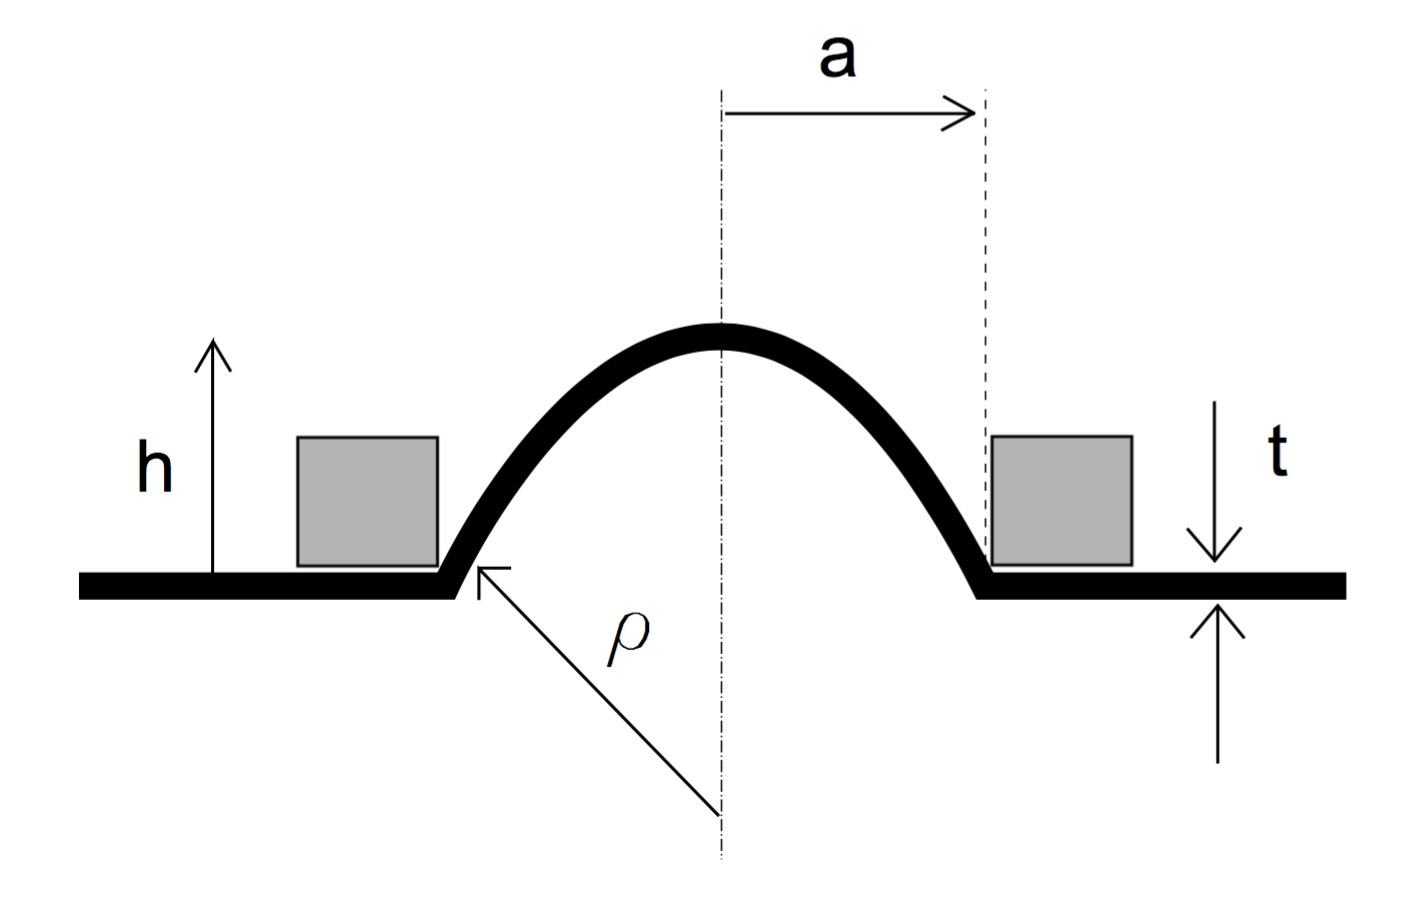
\includegraphics[width=4in]{hydroforming_sample.jpg} 
   \caption{Sheet Hydroforming Machine}
   \label{fig:example}
\end{figure}

\newpage

\begin{equation}
\rho = \frac{a^2+h^2}{2h}
\end{equation}
\bigskip

\begin{equation}
\bar{\sigma}=\frac{\rho}{4t_{o}}*\frac{a^2}{h}*\left[1+\left(\frac{h}{a}\right)^2\right]
\end{equation}
\bigskip

\begin{equation}
\frac{t_{o}}{t} = \frac{2\rho h}{a^2}
\end{equation}
\bigskip

\begin{equation}
\bar{\epsilon}=\epsilon_{\phi}=ln\frac{t_{o}}{t}
\end{equation}
\bigskip
\bigskip



The stress for each sample can also be calculated from the effective strain using the power law, shown in (5). The values for $K$ and $n$ from two different sources are shown in Table 1 and can be used with (5). One set of values is published [1], and the other set is obtained from a microscale tension test [2]. 
\bigskip


\begin{equation}
\sigma=K\epsilon^n
\end{equation}
\bigskip


\begin{center}
Table 1\\
Power law material properties for SS 304 \\
for annealed, 0.204 mm thick. \\
\begin{tabular}{ c c c}
\hline
 & n & K \\
 &    & (GPa)\\
\hline
Published[1] & 0.450 &.275\\
Microscale Tension Test [2] & 0.408 & 1.113\\
\hline
\end{tabular}
\end{center}
\bigskip
\bigskip


According to [3], using hydroforming in manufacturing is extremely beneficial. The cost is lower than traditional manufacturing processes and the parts end up being more light-weight with a higher stiffness to weight ratio. Using this method also provides seamless bonding in some applications, which results in stronger bonds than traditional methods such as welding. 
\bigskip
 


\newpage

\begin{figure}[htbp] %  figure placement: here, top, bottom, or page
   \centering
   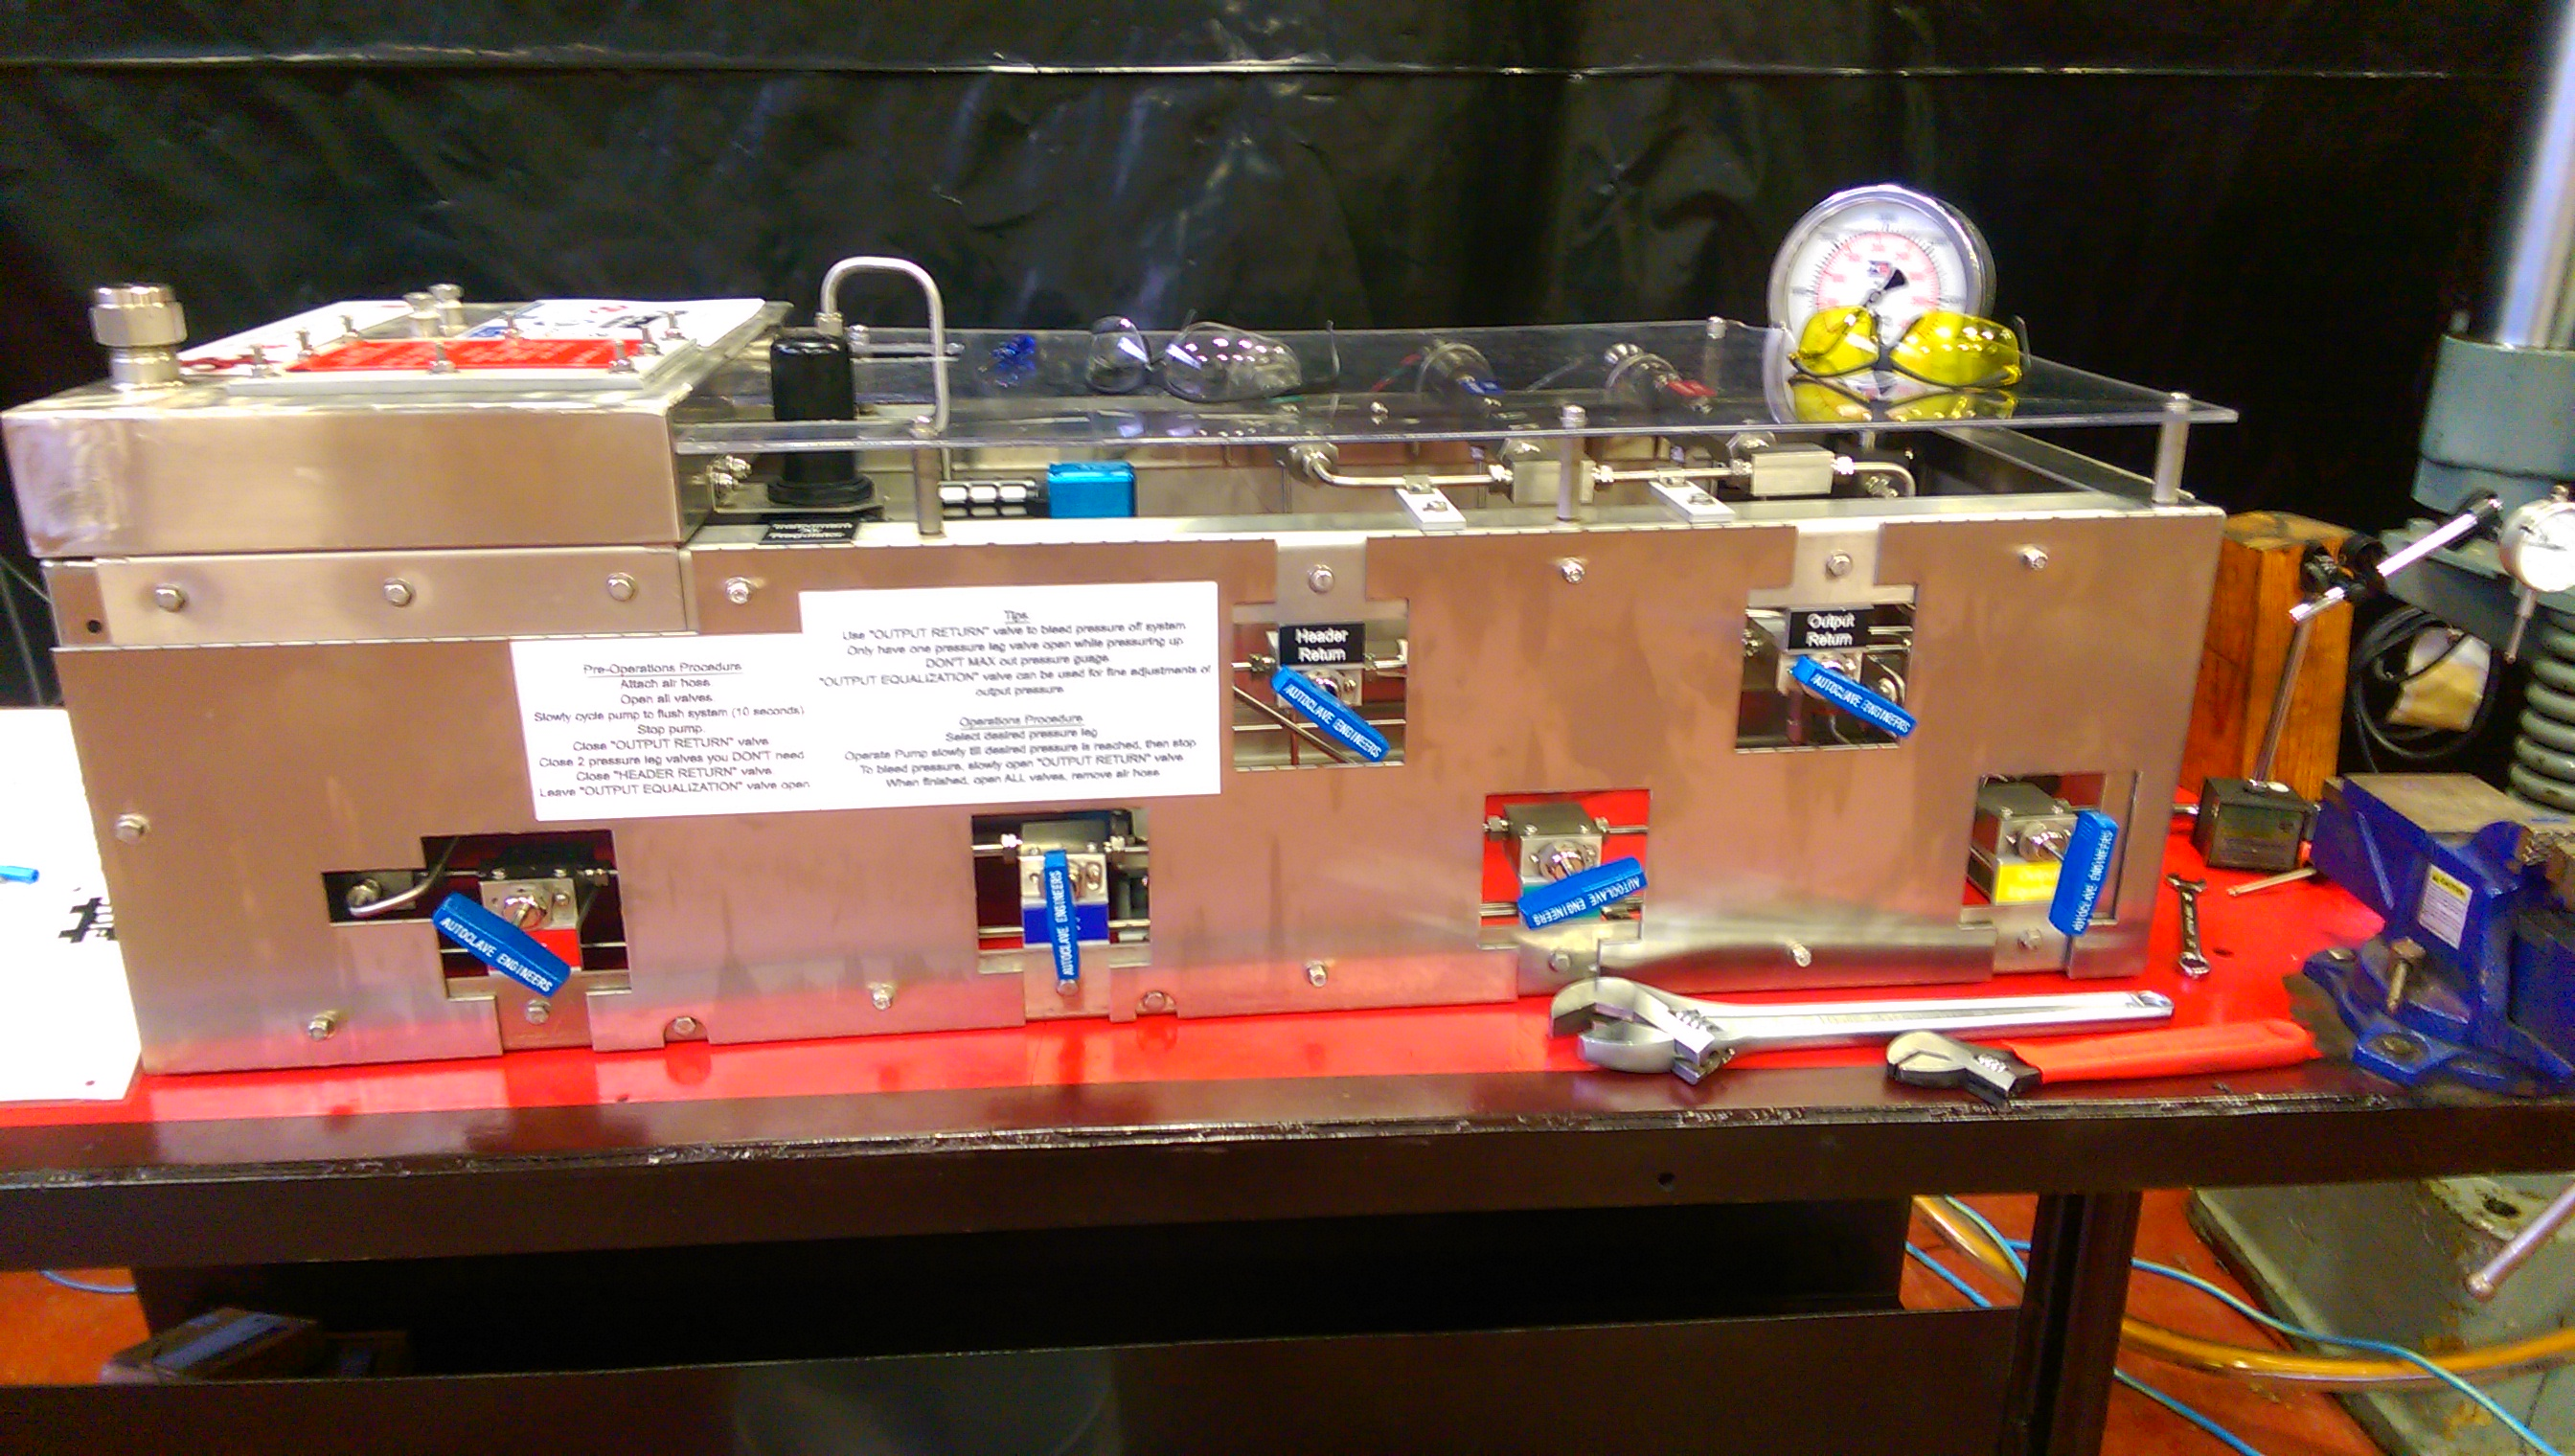
\includegraphics[width=5in]{IMAG00404.jpg} 
   \caption{Hydroforming Machine}
   \label{fig:example}
\end{figure}
\bigskip


\section*{\fontsize{12}{12}\selectfont PROCEDURE}
The sheet hydroforming test was conducted in the metal forming lab on campus. The equipment used was a hydroforming machine, shown in Figure 2, and a digital read-out caliper to measure the dome heights after tests. Twelve samples were tested, one by one, at varying pressures. The burst pressure was recorded for two samples, and all subsequent samples were tested in pairs at a pressure. Each sample's resulting dome height was measured, factoring in the original sample thickness to get the true dome height. 
\bigskip

The average dome height was plotted as a function of pressure and the linear relationship and $R^2$ value were determined. The actual height data was also plotted on the same graph to show how the average height compared to the data. The recorded data was used to calculate the effective stress and effective strain. The effective stress was plotted as a function of effective strain on a log-log graph and was fitted with a power-law trend line, for which the $R^2$ value was reported. The stress was then recalculated using the power law equation (5) for the effective strain values; once with the first set of $K$ and $n$ from Table 1, and again with the second set. These stress relations, as well as the effective stress relation, were then all plotted on a log-log graph as a function of strain.



\section*{\fontsize{12}{12}\selectfont RESULTS AND DISCUSSION}
The data recorded from the experiment is shown in Table 2. A plot of the average height as a function of pressure can be seen in Figure 3. Also included on the plot is a linear trend line along with its $R^2$ value, as well as the original height data. Using the equation for the trend line in Figure 3, the would-be dome height for the bursted samples can be predicted. The dome height for the sample which burst at 117.21 MPa would be about 1.8 mm, and the dome height for the sample that bursted at 110.32 MPa would be about 1.71 mm.
\bigskip



\newpage


% table2
\begin{center}
Table 2\\
Experiment Data\\
\begin{tabular}{ c c }
\hline
Pressure  & Dome Height \\
(MPa)     & (mm)        \\
\hline
117.211 & burst       \\
110.316 & burst       \\
96.527  & 1.551    \\
96.527  & 1.572    \\
82.737  & 1.365    \\
82.737  & 1.157    \\
68.948   & 1.164     \\
68.948   & 1.169     \\
48.263  & 0.944    \\
48.263  & 1.017    \\
27.579  & 0.552    \\
27.579 & 0.568     \\
\hline
\end{tabular}
\end{center}
\bigskip
\bigskip


\begin{figure}[h] %  figure placement: here, top, bottom, or page
   \centering
   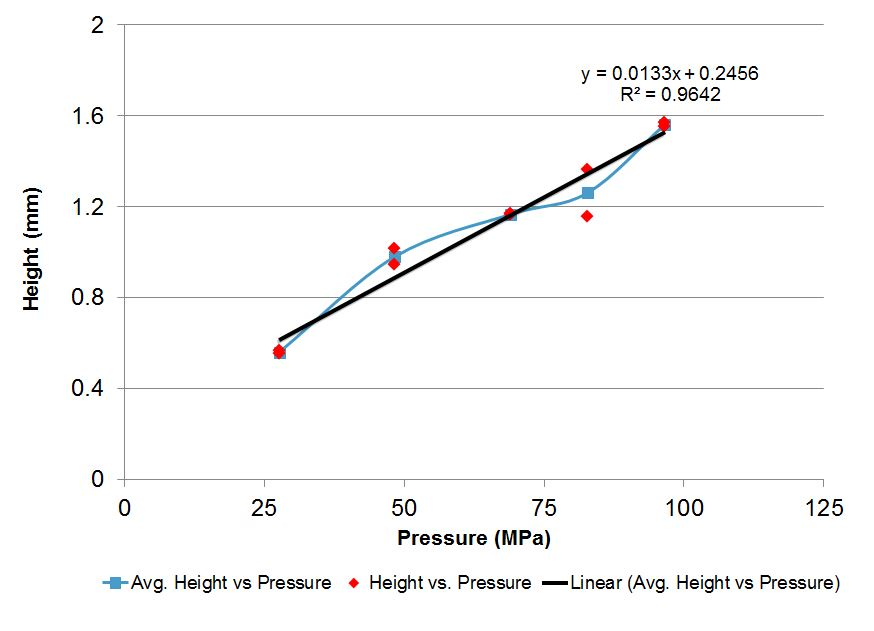
\includegraphics[width=5.5in,height=4in]{height_vs_pressure.jpg} 
   \caption{Height vs Pressure}
\end{figure}
\bigskip

\newpage

The effective stress is plotted as a function of effective strain on a log-log graph in Figure 4. This stress-strain relationship was calculated using the average heights plotted in Figure 3. Included on the plot is a power-law trend line along with its $R^2$ value. It should be noted that the power-law trend line appears linear on this plot because the slope of a power-law equation is logarithmic in nature. Also, note that if the maximum and/or minimum heights were used instead of the average heights for each pressure, the stress-strain relationship would differ.
\bigskip


The effective stress is plotted again on a log-log graph in Figure 5, along with the stresses calculated using the power-law equation (5) with the two sets of $K$ and $n$ in Table 1. Note that the the stresses calculated using the power-law relation have a slope which appears linear on a logarithmic scale because power-law relations have a slope which is logarithmic in nature. This differs from the experimental stress-strain relation because the experimental relation was calculated using methods that do not result in a relation with a logarithmic slope.
\bigskip
\bigskip



\begin{figure}[h] %  figure placement: here, top, bottom, or page
   \centering
   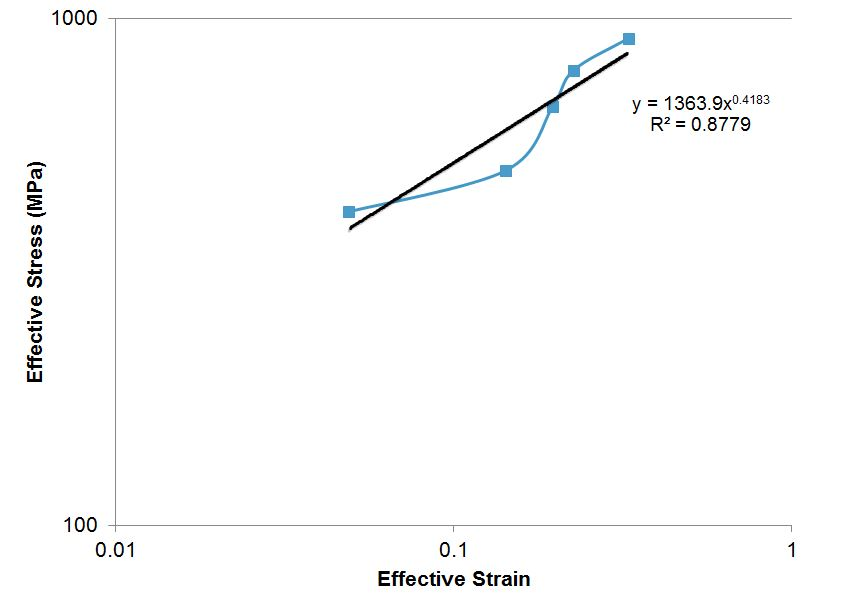
\includegraphics[width=6in,height=4.5in]{eff_stress_vs_strain.jpg} 
   \caption{Effective Stress vs Effective Strain (log-log)}
\end{figure}

\newpage

\begin{figure}[h!]
  \centering
    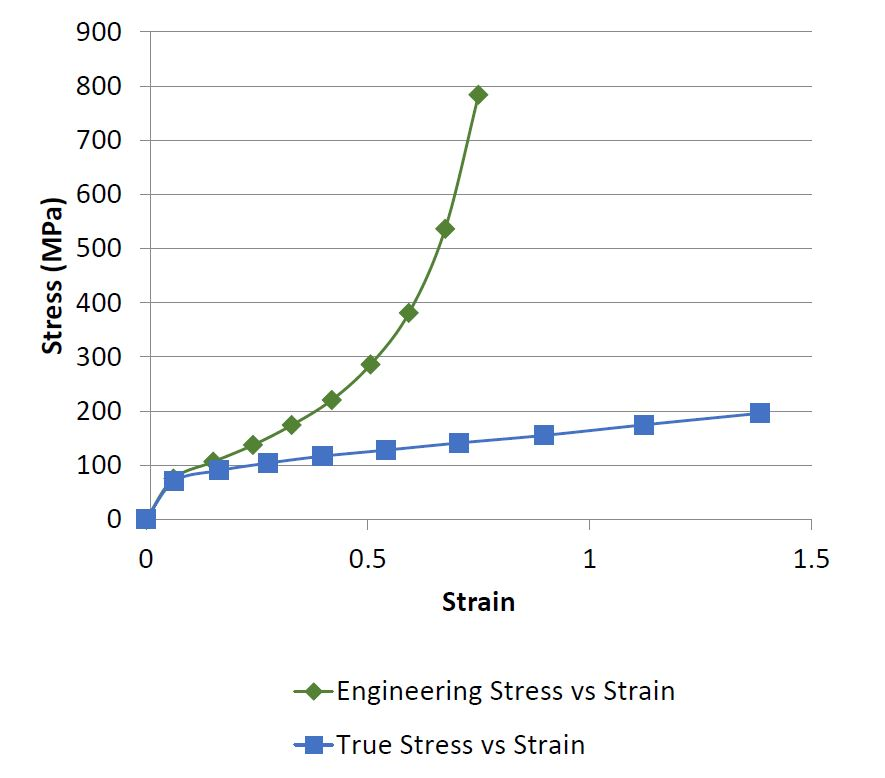
\includegraphics[width=6in,height=4.5in]{stress_vs_strain.jpg}
    \caption{Stresss vs Effective Strain}
\end{figure}


\section*{\fontsize{12}{12}\selectfont CONCLUSION}
The data from this sheet hydroforming test performed on UL campus has been analyzed and plotted. The originally recorded data was used to calculate the effective stress and strain, as well as the stresses calculated using the stress-strain power-law properties. The results were plotted and it was found that the effective stress closely matched a power-law trend. It was also seen that using power-law properties for obtaining stresses from strains results in a curve that appears linear on a log-log graph, which is because the slope of a power-law trend is logarithmic in nature. It should be noted that hydroforming is a practice that can greatly improve the manufacturing industry if more widely used; therefore, it is important to perform tests like these to advance the field in means of predicting the resulting geometry of different materials at different pressures.

\bigskip


\section*{\fontsize{12}{12}\selectfont REFERENCES}

\begin{thebibliography}{2}

\bibitem{Wagner}
Ng, K., Wagner, S.W., Camelio, J., Emblom, W.J. (2010). ?Experimental Analysis of Micro Tube
Hydroforming Process.? Transactions of NAMRC of SME, 38, 577-584.


\bibitem{Emblom}
Emblom, W.J., Ibne Islam, Md.F.S. Jones, R.J., Aithal, M., Wagner, S.W., 2015,
"Determining Material Properties of Annealed SS 304 Sheet Based on Multiscale
Hydroforming" Journal of Strain Analysis. 


\bibitem{AmericanHydroformers}
"Tube Hydroforming Step by Step Process," What is Hydroforming?, n.d., from:
http://www.americanhydroformers.com/what-is-hydroforming/
%\bibitem{McGinty}
%Mcginty, B., n.d.,
%"True Strain," \emph{Continuum Mechanics}, from
%http://www.continuummechanics.org/
%
%\bibitem{French}
%French, D., July 1991,
%"Creep and Creep Failures," from
%http://www.nationalboard.org/Index.aspx?pageID=181
%
%\bibitem{The Structure of Metals}
%n.d., "Closest-Packed Structures," \emph{The Structure of Materials}, from
%http://chemed.chem.purdue.edu/genchem/topicreview/bp/ch13/structure.php

\end{thebibliography}

%\section*{\fontsize{12}{12}\selectfont APPENDIX}

%\begin{table}[h!]
%  \caption{}
%  \includegraphics[width=\linewidth]{table1.png}
%\end{table}

\end{document}
----------------------------%TEmplates-------------------------------

-------------------------Figure-----------------------

\begin{figure}[h!]  
  \centering
    \includegraphics[width=\linewidth]{**file**}
    \caption{Docking Station}
\end{figure}

---------------------------Table-----------------------
\begin{table}[ht]
\caption{Nonlinear Model Results} % title of Table
\centering % used for centering table
\begin{tabular}{c c c c} % centered columns (4 columns)
\hline\hline %inserts double horizontal lines
Case & Method\#1 & Method\#2 & Method\#3 \\ [0.5ex] % inserts table
%heading
\hline % inserts single horizontal line
1 & 50 & 837 & 970 \\ % inserting body of the table
2 & 47 & 877 & 230 \\
3 & 31 & 25 & 415 \\
4 & 35 & 144 & 2356 \\
5 & 45 & 300 & 556 \\ [1ex] % [1ex] adds vertical space
\hline %inserts single line
\end{tabular}
\label{table:nonlin} % is used to refer this table in the text
\end{table}



probably best to insert as an image from excel

\bigskip\\
\begin{table}[h!]
  \caption{}
  \includegraphics[width=\linewidth]{**file**}
\end{table}
\bigskip\\





-----------------------------Equations------------------------
-----------------------------Regular
\begin{equation}
a = b + c
\end{equation}

--------------------------------- Multiline
\begin{multline}
a = b + c + d + e + f
+ g + h + i + j \\
+ k + l + m + n + o
\end{multline}

-------------------------------Citations-------------------------
\bibitem{Author last name}
  Last, First., year of publication,
  article name, book(etc) name, from \\
  link goes here

----------------------------------other-----------------------------

equations:
http://moser-isi.ethz.ch/docs/typeset_equations.pdf

citations:
http://library.missouri.edu/engineering/about/guides/asme
https://www.asme.org/shop/proceedings/conference-publications/references